%==============================================================================
% locality-performance.tex
%==============================================================================

\chapter{Performance Evaluation}
\label{chap:locality-performance}

\section{Methodology}
\label{sec:locality-performance-methodology}

The performance results in this chapter are obtained on an Intel
Nehalem system with 2 processors and 8 cores, running Ubuntu 9.04
64-bit with kernel 2.6.29 patched to support perfmon2
\cite{Eranian2008}.

The JVM used is Sun Hotspot JDK 1.6.0\_20 which is invoked with the
following parameters:

\begin{lstlisting}[style=Listing]
  -server -Xmx4096M -Xms4096M -Xss8M -XX:+UseNUMA
\end{lstlisting}

Appendix \ref{sec:experimental-setup-mafushi} gives a more detailed
description of the test machine.

Besides the runtime of the benchmarks, we are mostly interested in the
count of cache hits and miss events. Since the last level cache is
part of the uncore, we have to use the uncore PMU to count L3 cache
events. We use perfmon2 to track the following events
\cite{Levinthal2009}:

\begin{itemize}
\item \lstinline!UNC_LLC_HITS.READ!: Number of L3 cache read hits
\item \lstinline!UNC_LLC_MISS.READ!: Number of L3 cache read misses
\end{itemize}

The execution time reported is the average of the 3 best benchmark
iterations from 10 separate invocations. The cache events count
presented is that of the best benchmark execution from the same 10
invocations used to get the runtime.


\section{Non-Locality Benchmarks}
\label{sec:locality-performance-non-locality}

It is important that our new scheduler implementation does not affect
the performance of existing locality-ignorant intervals
applications. Thus, we run the locality-ignorant JGF benchmarks
(Appendix \ref{chap:benchmarks}) with our new scheduler
implementation. As Figure \ref{fig:locality-performance-jgf} shows,
the performance of locality-ignorant JGF benchmarks on the
locality-aware intervals scheduler is comparable to the original
implementation.

\begin{figure}[!ht]
  \centering
  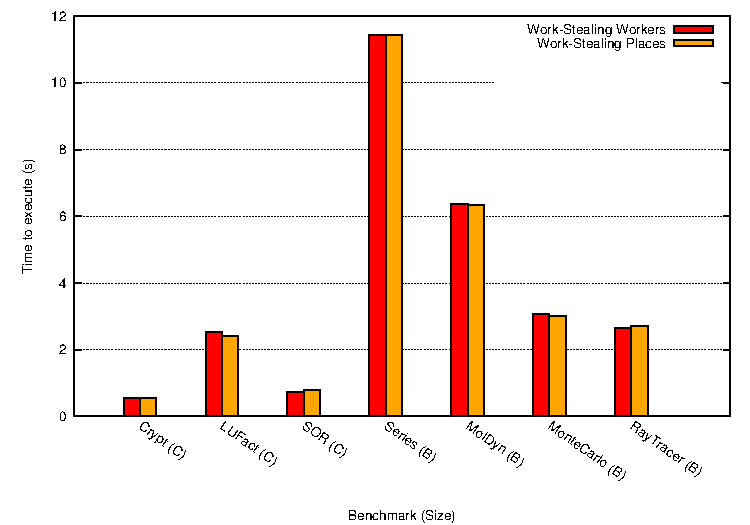
\includegraphics[width=0.8\linewidth]{locality-performance/mafushi-jgf}
  \caption[Locality-ignorant JGF benchmarks running on locality-aware
  scheduler]{Locality-ignorant JGF benchmarks using the locality-aware
    scheduler on our Intel Nehalem (Appendix
    \ref{sec:experimental-setup-mafushi}) test machine}
  \label{fig:locality-performance-jgf}
\end{figure}


\section{Locality Benchmarks}
\label{sec:locality-performance-locality}

\subsection{Cache-Stress Test}
\label{sec:locality-performance-cache-stress-test}

The \emph{Cache Stress Test} benchmark was ported over from the
threaded version to intervals (Chapter \ref{chap:locality-approach}).

It first randomly initializes two integer arrays of equal size as the
last level cache per processor. The root interval creates 64
subintervals with their locality set to a specific place: 32 have
their locality set for \emph{place 0} and 32 for \emph{place 1}.

One half of the intervals operate on the elements of the first array
and the other half operate on the elements of the second array. Each
interval's task adds and multiplies all the elements of its respective
array 100 times.

Like in the threaded version, we implement several different variants
of the benchmark, each having different locality properties:

\begin{description}
\item[Best Locality:] All the intervals working on the first array
  have their locality set to \emph{place 0} and all intervals working
  on the second array have their locality set to \emph{place 1}.
\item[Ignorant Locality:] The intervals do not have any locality set.
\item[Random Locality:] The locality of the intervals is set to a
  \emph{random} place.
\item[Worst Locality:] Half the intervals with locality for
  \emph{place 0} work on the first array, and the other half works on
  the second array and vice versa for the intervals with locality for
  \emph{place 1}.
\end{description}

Table \ref{tab:locality-performance-cache-stress-test} shows the
execution times and the speedups over the sequential algorithm for the
different benchmark implementations. Like in the threaded version, the
implementation with \emph{best locality} is the fastest and provides
the largest speedup. Due to load-balancing of the work-stealing
places, the difference between the various localities it not that big
as in the threaded benchmark implementations.

\begin{table}[htb]
  \centering
  \begin{tabular}{ln{2}{3}n{1}{2}}
    \toprule
    & {Runtime (in seconds)} & {Speedup (over sequential)} \\\midrule
    \emph{Best Locality} & 3.596 & 7.11 \\
    \emph{Ignorant Locality} & 4.038 & 6.33 \\
    \emph{Random Locality} & 4.030 & 6.35 \\
    \emph{Worst Locality} & 3.982 & 6.42 \\
    \emph{Sequential Implementation}\hspace{0.5cm} & 25.571 & 1 \\\bottomrule
  \end{tabular}
  \caption{\emph{Cache Stress Test} execution times and speedups over sequential implementation}
  \label{tab:locality-performance-cache-stress-test}
\end{table}

Figure \ref{fig:locality-performance-cache-stress-test} illustrates
the execution times normalized to that of the \emph{best locality}
implementation. The \emph{best locality} implementation shows a
speedup over the other locality benchmarks of about 1.1\texttimes.

\begin{figure}[!ht]
  \centering
  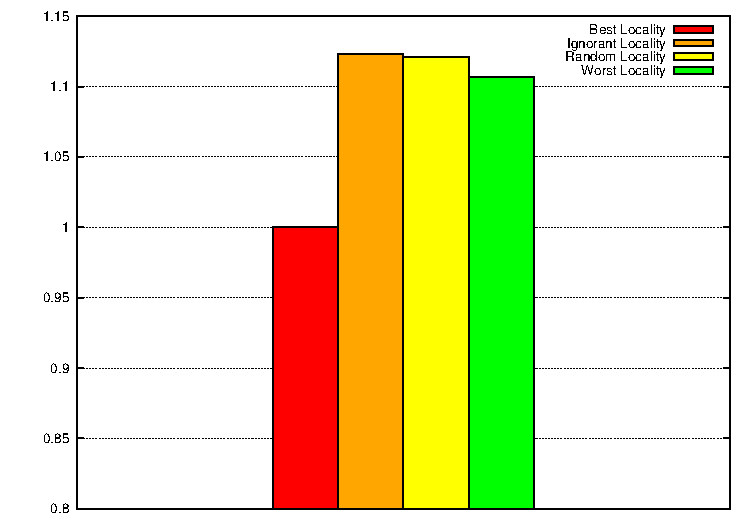
\includegraphics[width=0.7\linewidth]{locality-performance/cache-stress-test}
  \caption{\emph{Cache Stress Test} with execution times normalized to
    \emph{best locality}}
  \label{fig:locality-performance-cache-stress-test}
\end{figure}

Table \ref{tab:locality-performance-cache-stress-test-cache-misses}
lists the number of L3 cache read misses and hits. In Figure
\ref{fig:locality-performance-cache-stress-test} they are shown
normalized to the measurements of the \emph{best locality}
implementation. The \emph{best locality} benchmark has up to
3.1\texttimes\ fewer L3 cache read misses than the other
benchmarks. Compared to the other benchmarks, it has almost
1.5\texttimes\ more L3 cache read hits.

\begin{table}[htb]
  \centering
  \begin{tabular}{ln{4}{0}n{4}{0}}
    \toprule
    & {L3 Cache Read Misses} & {L3 Cache Read Hits} \\\midrule
    \emph{Best Locality}\hspace{1cm} & 275 & 2335 \\
    \emph{Ignorant Locality} & 837 & 1568 \\
    \emph{Random Locality} & 854 & 1570 \\
    \emph{Worst Locality} & 837 & 1539 \\\bottomrule
  \end{tabular}
  \caption[\emph{Cache Stress Test} L3 cache read misses and hits]
  {\emph{Cache Stress Test} L3 cache read misses and hits (rounded to the nearest million)}
  \label{tab:locality-performance-cache-stress-test-cache-misses}
\end{table}

\begin{figure}[!ht]
  \centering
  \subfloat[L3 Cache Read Misses]{
    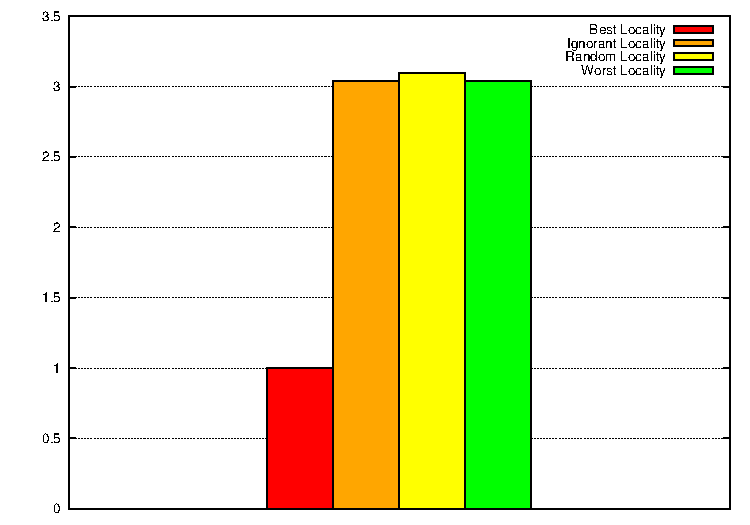
\includegraphics[width=0.5\linewidth]{locality-performance/cache-stress-test-cache-misses}
    \label{fig:locality-performance-cache-stress-test-cache-misses}
  }
  \subfloat[L3 Cache Read Hits]{
    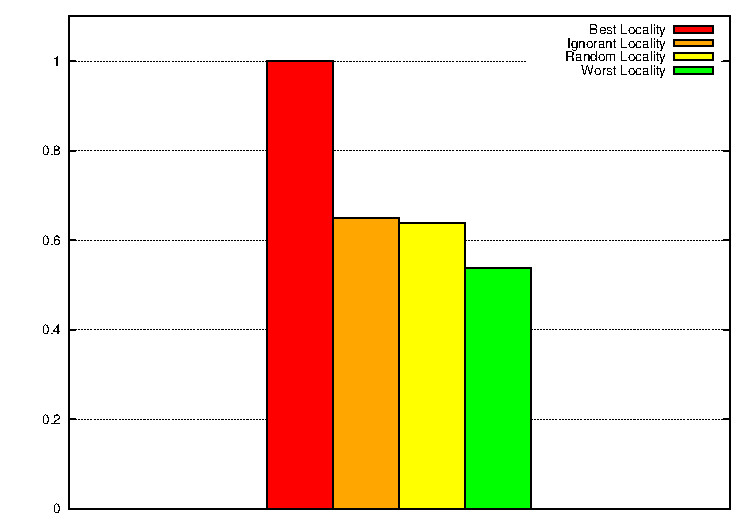
\includegraphics[width=0.5\linewidth]{locality-performance/cache-stress-test-cache-hits}
    \label{fig:locality-performance-cache-stress-test-cache-hits}
  }
  \caption{\emph{Cache Stress Test} with L3 cache read misses and hits
    normalized to \emph{best locality}}
  \label{fig:locality-performance-cache-stress-test-cache}
\end{figure}

Our locality-aware intervals scheduler preserves the properties of the
threaded version of the \emph{Cache Stress Test} benchmark.

% \subsection{Merge Sort}
% \label{sec:locality-performance-merge-sort}

% \emph{Merge Sort} is representative of many programs that use a
% recursive divide-and-conquer paradigm. Our \emph{Merge Sort} benchmark...

% The \emph{Block Matrix Multiplication} benchmark multiplies two $n
% \times n$ matrices $A$ and $B$ using locality-aware intervals. The
% implementation employs the following recursion to calculate the matrix
% $C$:

% \begin{eqnarray*}
%   \begin{pmatrix}
%     C_{00} & C_{01} \\
%     C_{10} & C_{11}
%   \end{pmatrix}
%   &
%   =
%   &
%   \begin{pmatrix}
%     A_{00} & A_{01} \\
%     A_{10} & A_{11}
%   \end{pmatrix}
%   \cdot
%   \begin{pmatrix}
%     B_{00} & B_{01} \\
%     B_{10} & B_{11}
%   \end{pmatrix}
%   \\
%   &
%   =
%   &
%   \begin{pmatrix}
%     A_{00} \cdot B_{00} + A_{01} \cdot B_{10} & A_{00} \cdot B_{01} + A_{01} \cdot B_{11} \\
%     A_{10} \cdot B_{00} + A_{11} \cdot B_{10} & A_{10} \cdot B_{01} + A_{11} \cdot B_{11} \\
%   \end{pmatrix}
% \end{eqnarray*}

% Now the $n \times n$ matrix multiplication can be reduced to 8
% multiplications and 4 additions of $(n/2) \times (n/2)$
% submatrices. The 8 multiplications can be calculated in parallel and
% when they are done, the 4 additions can be computed in parallel too.

% We run the \emph{Block Matrix Multiplication} benchmark to multiply
% two random $2048 \times 2048$ matrices. A $2048 \times 2048$ matrix
% needs about 16 MB of memory and should just fits in the L3 caches of
% the two processors of our test machine. The benchmark recursively
% splits the $2048 \times 2048$ matrices $A$ and $B$ into quadrants
% until they reach size $32 \times 32$.

% We implement two variants of the benchmark: \emph{best locality} and
% \emph{worst locality}. Figure
% \ref{fig:locality-performance-block-matrix-multiplication-locality}
% shows the division of matrix quadrants between places.

% The \emph{best locality} benchmark runs all addition and
% multiplication intervals of the matrix quadrants 0 and 3 in
% \emph{place 0} and and the ones of the quadrants 1 and 2 in
% \emph{place 1}. This way the places are able to share their local L3
% cache in an efficient way.

% The \emph{worst locality} benchmark runs the multiplication and
% addition intervals on different places.

% \begin{figure}[!ht]
%   \centering
%   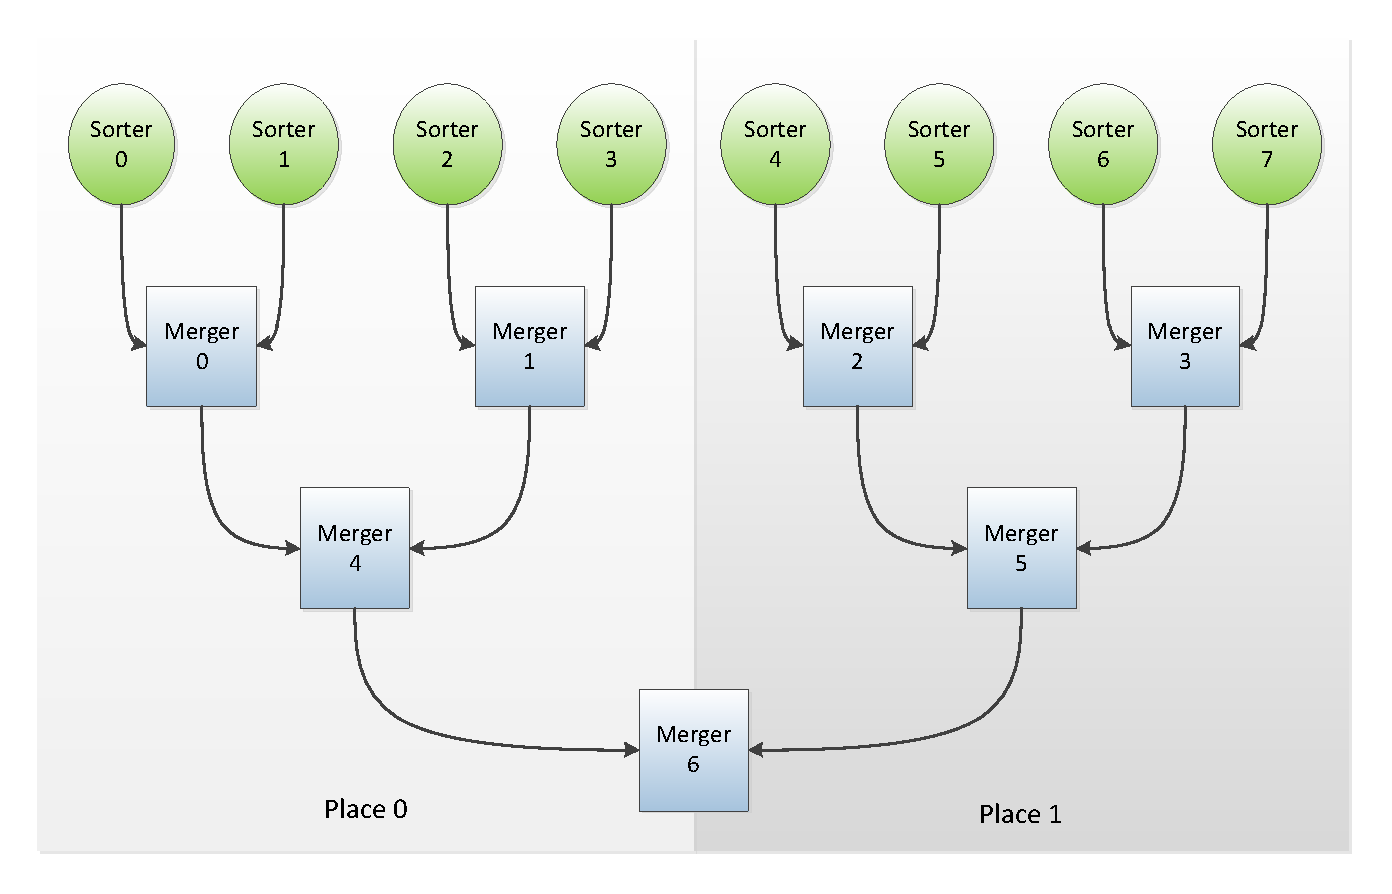
\includegraphics[width=\linewidth]{locality-performance/mergesort}
%   \caption{Merge Sort: Best locality}
%   \label{fig:locality-performance-mergesort}
% \end{figure}

% Table \ref{tab:locality-performance-block-matrix-multiplication} shows
% the execution times and the speedups over the sequential algorithm for
% the \emph{best locality} and \emph{worst locality} benchmark
% implementations. The implementation with \emph{best locality} is the
% fastest and provides the largest speedup.

% \begin{table}[htb]
%   \centering
%   \begin{tabular}{ln{2}{3}n{1}{2}}
%     \toprule
%     & {Runtime (in seconds)} & {Speedup (over sequential)} \\\midrule
%     \emph{Best Locality} & 4.690 & 3.97 \\
%     \emph{Worst Locality} & 5.399 & 3.45 \\
%     \emph{Sequential Implementation}\hspace{0.5cm} & 18.632 & 1 \\\bottomrule
%   \end{tabular}
%   \caption{\emph{Block Matrix Multiplication} execution times and speedups over sequential implementation}
%   \label{tab:locality-performance-block-matrix-multiplication}
% \end{table}

% Figure \ref{fig:locality-performance-block-matrix-multiplication}
% illustrates the execution times normalized to that of the \emph{best
%   locality} implementation. The \emph{best locality} implementation
% shows a speedup over the \emph{worst locality} of about
% 1.15\texttimes.

% \begin{figure}[!ht]
%   \centering
%   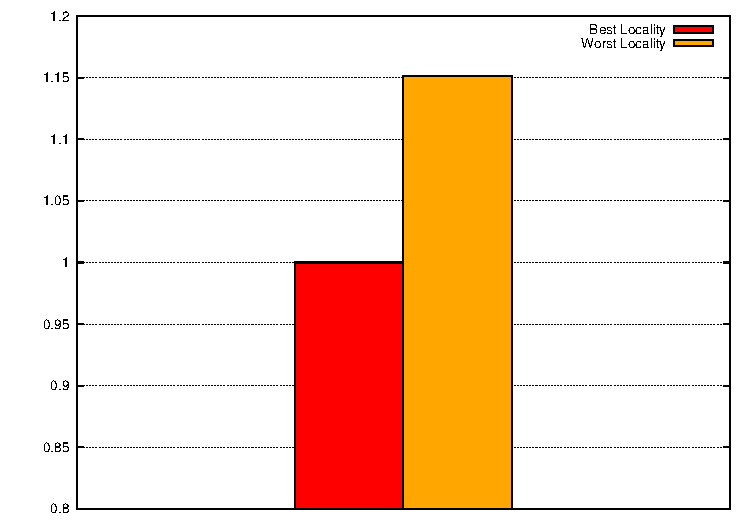
\includegraphics[width=0.7\linewidth]{locality-performance/block-matrix-multiplication}
%   \caption{\emph{Block Matrix Multiplication} with execution times normalized to
%     \emph{best locality}}
%   \label{fig:locality-performance-block-matrix-multiplication}
% \end{figure}

% Table \ref{tab:locality-performance-block-matrix-multiplication-cache-misses}
% lists the number of L3 cache read misses and hits. In Figure
% \ref{fig:locality-performance-block-matrix-multiplication} they are shown
% normalized to the measurements of the \emph{best locality}
% implementation. The \emph{best locality} benchmark has up to
% 3.1\texttimes\ fewer L3 cache read misses than the other
% benchmarks. Compared to the other benchmarks, it has almost
% 1.5\texttimes\ more L3 cache read hits.

% \begin{table}[htb]
%   \centering
%   \begin{tabular}{ln{4}{0}n{4}{0}}
%     \toprule
%     & {L3 Cache Read Misses} & {L3 Cache Read Hits} \\\midrule
%     \emph{Best Locality}\hspace{1cm} & 360 & 1461 \\
%     \emph{Worst Locality} & 476 & 1273 \\\bottomrule
%   \end{tabular}
%   \caption[\emph{Block Matrix Multiplication} L3 cache read misses and hits]
%   {\emph{Block Matrix Multiplication} L3 cache read misses and hits (rounded to the nearest million)}
%   \label{tab:locality-performance-block-matrix-multiplication-cache-misses}
% \end{table}

% \begin{figure}[!ht]
%   \centering
%   \subfloat[L3 Cache Read Misses]{
%     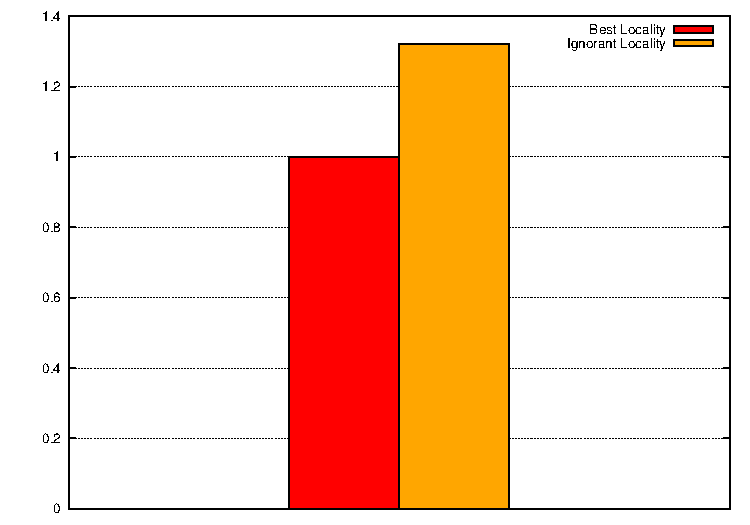
\includegraphics[width=0.5\linewidth]{locality-performance/block-matrix-multiplication-cache-misses}
%     \label{fig:locality-performance-block-matrix-multiplication-cache-misses}
%   }
%   \subfloat[L3 Cache Read Hits]{
%     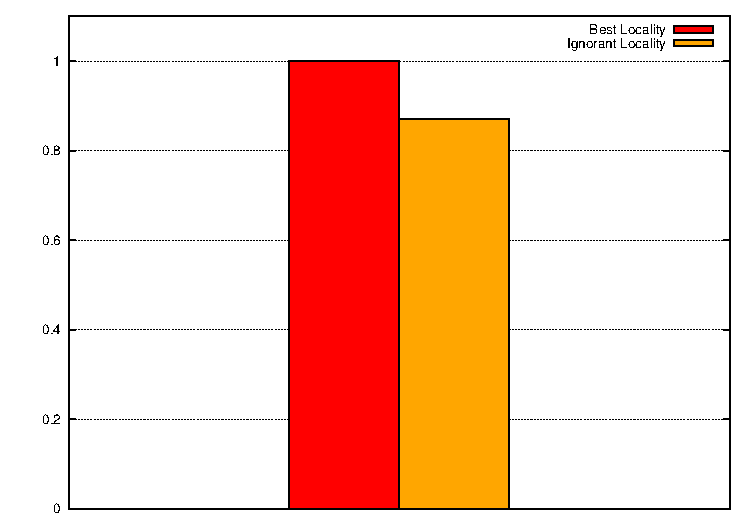
\includegraphics[width=0.5\linewidth]{locality-performance/block-matrix-multiplication-cache-hits}
%     \label{fig:locality-performance-block-matrix-multiplication-cache-hits}
%   }
%   \caption{\emph{Block Matrix Multiplication} with L3 cache read misses and hits
%     normalized to \emph{best locality}}
%   \label{fig:locality-performance-block-matrix-multiplication-cache}
% \end{figure}

% \todo{Describe benchmark ``Merge Sort''}

\subsection{Block Matrix Multiplication}
\label{sec:locality-performance-block-matrix-multiplication}

The \emph{Block Matrix Multiplication} benchmark multiplies two $n
\times n$ matrices $A$ and $B$ using locality-aware intervals. The
implementation employs the following recursion to calculate the matrix
$C$:

\begin{eqnarray*}
  \begin{pmatrix}
    C_{00} & C_{01} \\
    C_{10} & C_{11}
  \end{pmatrix}
  &
  =
  &
  \begin{pmatrix}
    A_{00} & A_{01} \\
    A_{10} & A_{11}
  \end{pmatrix}
  \cdot
  \begin{pmatrix}
    B_{00} & B_{01} \\
    B_{10} & B_{11}
  \end{pmatrix}
  \\
  &
  =
  &
  \begin{pmatrix}
    A_{00} \cdot B_{00} + A_{01} \cdot B_{10} & A_{00} \cdot B_{01} + A_{01} \cdot B_{11} \\
    A_{10} \cdot B_{00} + A_{11} \cdot B_{10} & A_{10} \cdot B_{01} + A_{11} \cdot B_{11} \\
  \end{pmatrix}
\end{eqnarray*}

Thus, the $n \times n$ matrix multiplication can be reduced to 8
multiplications and 4 additions of $(n/2) \times (n/2)$
submatrices. The 8 multiplications can be calculated in parallel and
when they are done, the 4 additions can be computed in parallel too.

We run the \emph{Block Matrix Multiplication} benchmark to multiply
two random $2048 \times 2048$ matrices. A $2048 \times 2048$ matrix
needs about 16 MB of memory and should just about fit in the L3 cache
of the two processors of our test machine. The benchmark recursively
splits the $2048 \times 2048$ matrices $A$ and $B$ into quadrants
until they reach size $32 \times 32$ and are multiplied using the
well-known sequential matrix multiplication algorithm.

We implement two variants of the benchmark: \emph{best locality} and
\emph{worst locality}. Figure
\ref{fig:locality-performance-block-matrix-multiplication-locality}
shows the division of matrix quadrants between places for both
variants:

\begin{description}
\item[Best Locality:] The \emph{best locality} benchmark runs all
  addition and multiplication intervals of the matrix quadrants 0 and
  3 in \emph{place 0} and and the ones of the quadrants 1 and 2 in
  \emph{place 1}. This way the places are able to share their local L3
  cache in an efficient way.
\item[Worst Locality:] The \emph{worst locality} benchmark runs the
  multiplication and addition intervals in different places destroying
  cache locality.
\end{description}

\begin{figure}[!ht]
  \centering
  \subfloat[Best Locality]{
    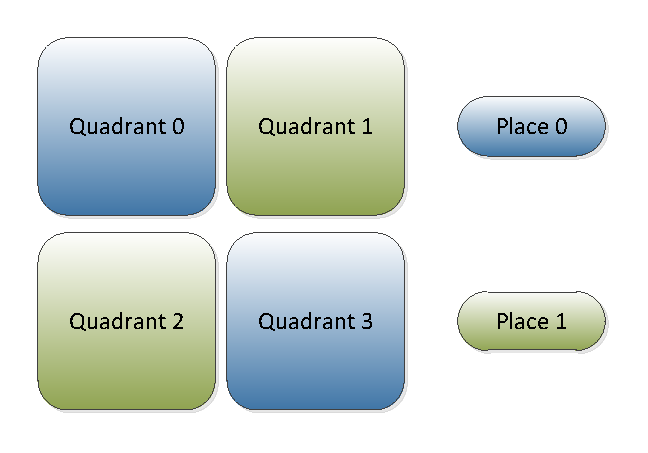
\includegraphics[width=0.5\linewidth]{locality-performance/block-matrix-multiplication-best-locality}
    \label{fig:locality-performance-block-matrix-multiplication-best-locality}
  }
  \subfloat[Worst Locality]{
    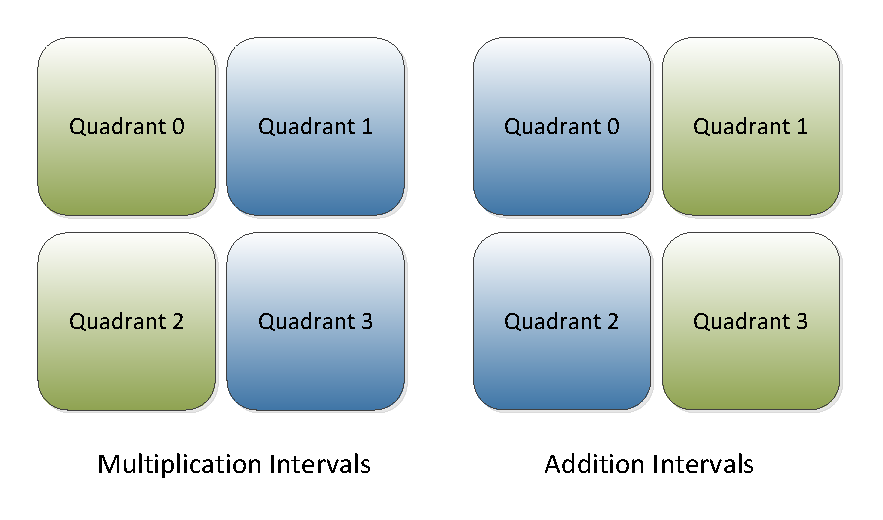
\includegraphics[width=0.5\linewidth]{locality-performance/block-matrix-multiplication-worst-locality}
    \label{fig:locality-performance-block-matrix-multiplication-worst-locality}
  }
  \caption{\emph{Block Matrix Multiplication} quadrants with \emph{best} and \emph{worst locality}}
  \label{fig:locality-performance-block-matrix-multiplication-locality}
\end{figure}

Table \ref{tab:locality-performance-block-matrix-multiplication} shows
the execution times and the speedups over the sequential algorithm for
the \emph{best locality} and \emph{worst locality} benchmark
implementations. The implementation with \emph{best locality} is the
fastest and provides the largest speedup.

\begin{table}[htb]
  \centering
  \begin{tabular}{ln{2}{3}n{1}{2}}
    \toprule
    & {Runtime (in seconds)} & {Speedup (over sequential)} \\\midrule
    \emph{Best Locality} & 4.690 & 3.97 \\
    \emph{Worst Locality} & 5.399 & 3.45 \\
    \emph{Sequential Implementation}\hspace{0.5cm} & 18.632 & 1 \\\bottomrule
  \end{tabular}
  \caption{\emph{Block Matrix Multiplication} execution times and speedups over sequential implementation}
  \label{tab:locality-performance-block-matrix-multiplication}
\end{table}

Figure \ref{fig:locality-performance-block-matrix-multiplication}
illustrates the execution time of the \emph{worst locality}
implementation normalized to that of the \emph{best locality}
implementation. The \emph{best locality} implementation shows a
speedup over the \emph{worst locality} of about 1.15\texttimes.

\begin{figure}[!ht]
  \centering
  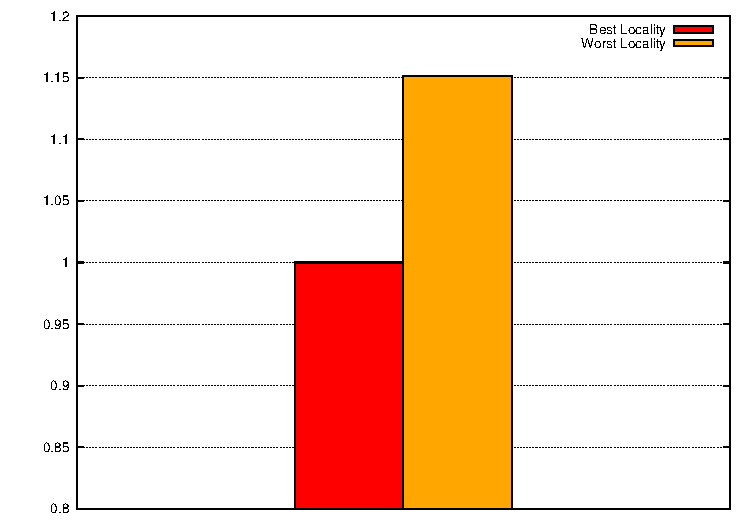
\includegraphics[width=0.65\linewidth]{locality-performance/block-matrix-multiplication}
  \caption{\emph{Block Matrix Multiplication} with execution times normalized to
    \emph{best locality}}
  \label{fig:locality-performance-block-matrix-multiplication}
\end{figure}

Table
\ref{tab:locality-performance-block-matrix-multiplication-cache-misses}
lists the number of L3 cache read misses and hits. In Figure
\ref{fig:locality-performance-block-matrix-multiplication} they are
shown normalized to the measurements of the \emph{best locality}
implementation. The \emph{best locality} benchmark has up to
1.3\texttimes\ fewer L3 cache read misses than the other
benchmarks. Compared to the other benchmarks, it has 1.15\texttimes\
more L3 cache read hits.

\begin{table}[htb]
  \centering
  \begin{tabular}{ln{4}{0}n{4}{0}}
    \toprule
    & {L3 Cache Read Misses} & {L3 Cache Read Hits} \\\midrule
    \emph{Best Locality}\hspace{1cm} & 360 & 1461 \\
    \emph{Worst Locality} & 476 & 1273 \\\bottomrule
  \end{tabular}
  \caption[\emph{Block Matrix Multiplication} L3 cache read misses and hits]
  {\emph{Block Matrix Multiplication} L3 cache read misses and hits (rounded to the nearest million)}
  \label{tab:locality-performance-block-matrix-multiplication-cache-misses}
\end{table}

\begin{figure}[!ht]
  \centering
  \subfloat[L3 Cache Read Misses]{
    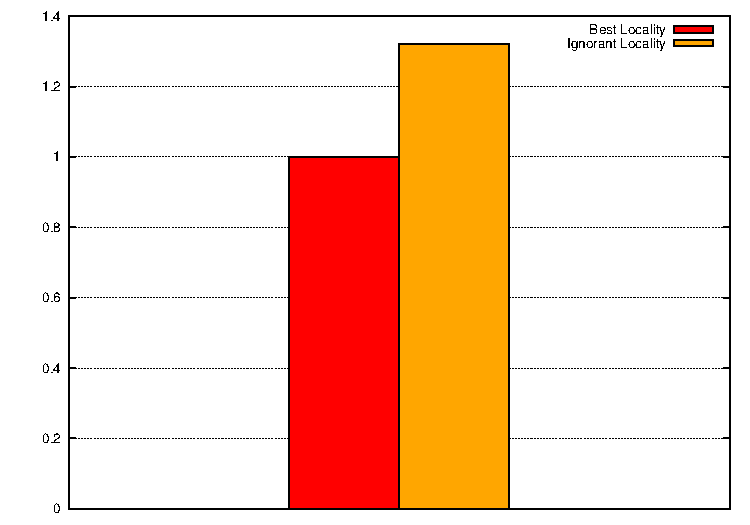
\includegraphics[width=0.5\linewidth]{locality-performance/block-matrix-multiplication-cache-misses}
    \label{fig:locality-performance-block-matrix-multiplication-cache-misses}
  }
  \subfloat[L3 Cache Read Hits]{
    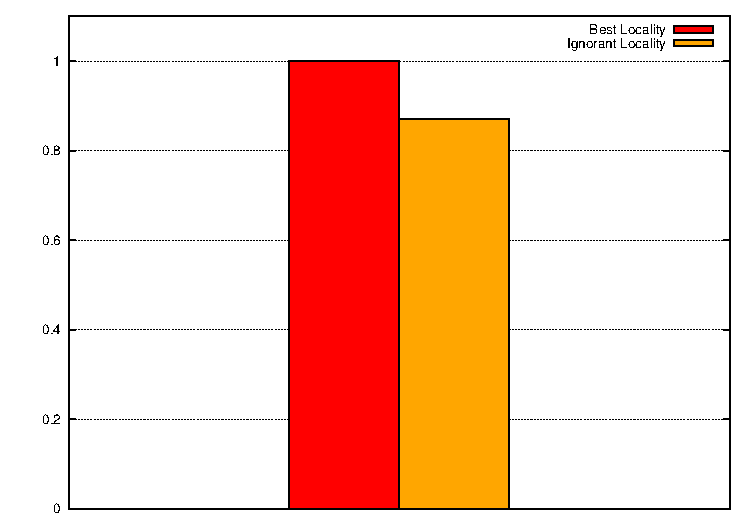
\includegraphics[width=0.5\linewidth]{locality-performance/block-matrix-multiplication-cache-hits}
    \label{fig:locality-performance-block-matrix-multiplication-cache-hits}
  }
  \caption{\emph{Block Matrix Multiplication} with L3 cache read misses and hits
    normalized to \emph{best locality}}
  \label{fig:locality-performance-block-matrix-multiplication-cache}
\end{figure}


%%% Local Variables: 
%%% mode: latex
%%% TeX-master: "thesis"
%%% End: 
